\subsection{Termine}
\label{termine}
Gerade in der Anfangszeit des Studiums gibt es eine Menge zu tun. Damit ihr
nicht das Wichtigste verpasst, haben wir die ersten Termine kompakt f"ur
euch zusammengefasst. Die meisten davon bieten die Gelegenheit Fragen zu
stellen und nebenbei gleich ein paar nette Kommilitonen kennen zu lernen.

Falls ihr es euch nicht schon gedacht habt: Die Spalten B und M geben an,
ob der Termin für Bachelor- oder Masterstudenten gedacht ist. Falls jemand
von euch den eigentlichen Termin verpasst, kann er meist ersatzweise auch
zum anderen erscheinen.

\end{multicols}
\begin{tabular}{|l|l|p{6.7cm}|c|c|c|}
\hline \textbf{Datum} 		& \textbf{Uhrzeit} 	& \textbf{Veranstaltung}						& \textbf{Ort} 	& \textbf{B}	& \textbf{M} 	\\
\hline 26.09. – 30.09.		& 1. Tag: 10:00	 	& Vorkurs Informatik							& PK 2.1		& B				& 				\\
	   17.10. – 21.10.		& 					& 												& 				& 				&    			\\
\hline Mo, 24.10. 			& 09:00 – 10:00		& Begrüßung	durch den Präsidenten				& Stadion		& B				& M				\\ 
\hline 						& 10:00 – 12:00	 	& Infobörse										& Altgebäude	& B				& M				\\
\hline   					& 10:30 – 12:00	 	& Begrüßung (M) \newline durch den Studiendekan	& IZ 160		& 				& M				\\
\hline 						& 13:30 – 15:00	 	& Begrüßung (B) \newline durch den Studiendekan	& PK 11.3		& B				& 				\\
\hline 						& 15:00 – 16:30		& Erste Vorlesung ,,Programmieren 1''			& SN 19.1		& B 			&				\\
\hline Di, 25.10.			& 10:00 – 11:45 	& Erstsemester-Frühstück 						& IZ Plaza 		& B 			& M 			\\ 
\hline 						& 12:00 – 13:30 * 	& FG-Einführung und \newline Stundenplan-Bauen 	& ??? * 		& B 			&  				\\%& ??? * & B &\\
\hline 						& 12:00 – 13:30 * 	& FG-Einführung und \newline Stundenplan-Bauen 	& IZ 160 * 		& 				& M				\\
\hline 						& 13:30 – 15:00 	& Rundgang mit den  Tutorengruppen 				& IZ 160 		& B 			& M				\\
\hline Mi, 26.10.			& 10:00 – 17:00		& Studium Generale								& Altgebäude	& B				& M 			\\
\hline Do, 03.11. 			& 19:00 			& Kneipentour der Fachgruppe 					& IZ 150 		& B 			& M				\\
\hline Mi, 09.11.	 		& 19:00 			& Spieleabend der Fachgruppe 					& vor  150 		& B 			& M				\\
\hline
\end{tabular} 

%%% Local Variables: 
%%% mode: latex
%%% TeX-master: "../../1-te"
%%% End: 

\begin{multicols}{2}

Zum besseren Verständnis der Spalte \textit{Ort} schau in den Abschnitt \textit{Campuskarte} auf Seite \pageref{campuskarte}.

%TODO folgendes muss dann aber auch wirklich umgesetzt werden:
Ihr findet die Termine auch online unter \url{http://fginfo.cs.tu-bs.de/index.php/termine/}.
Falls ihr einen Dienst, ein Handy oder eine Software nutzt, die das iCalender-Format unterstützt
könnt ihr die Termine auch von dort aus einbinden und habt sie somit im Blick. 
Dazu gehören z.\,B. iPhone, Android, Google Calendar, Outlook\,\dots. Eine Liste 
von ca. 60 Programmen findet ihr unter 
\url{http://en.wikipedia.org/wiki/List_of_applications_with_iCalendar_support}


% TODO es wäre schön, hier zu jedem Termin noch ein oder zwei Sätze zu schreiben, damit man sich darunter etwas vorstellen kann, ähnlich wie bei der TODO-Liste, wo ja auch diverse Textabschnitte folgen.

%In der \textit{Ort}-Spalte stehen meist Raumnummern. F"ur alle R"aume die nicht
%im IZ (steht f"ur Informatikzentrum) liegen, schaut am besten auf den
%Campusplan im Einband. Bei den R"aumen im IZ ist die erste Zahl das Stockwerk, f"ur
%den Rest m"usst ihr dann auf den Plan im Stockwerk schauen (Kleine Falle:
%zwischen EG und 1. OG liegt das Galeriegescho"s - Raum IZ 150 liegt also
%effektiv in der zweiten Etage).
% - Gl"uhweinabend im Informatikzentrum (IZ)

% Dieser Trick hilft uns, eine neue Seite zu erzwingen
% (auf diese passt eh nix sinnvolles mehr) und dennoch die 
% Spaltenlängen auszubalancieren.
\end{multicols}
    \begin{center}
          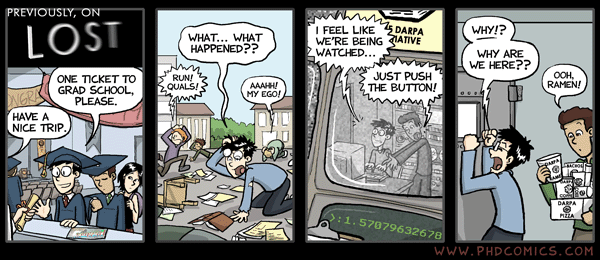
\includegraphics[width=\linewidth]
	  {bilder/comics/phd092706s.png}    \end{center}
\newpage
\begin{multicols}{2}

